\documentclass{beamer}
%packages
\usepackage[latin1]{inputenc}
\usepackage{graphicx}
\usepackage{hyperref}
\usepackage[english]{babel}

\hypersetup{urlcolor=red,colorlinks}
\definecolor{bg}{rgb}{0.95,0.95,0.95}
\usetheme{Rochester}

\title{XAPPY Project}
\author{xapi-team}
\institute{Institute for Computer Science, Free University Berlin}
\date{15.7.2011}
\begin{document}

\begin{frame}
	\titlepage
\end{frame}

\begin{frame}
	\tableofcontents
\end{frame}

%%%%%%%%%%%%%%%%%%%%%%

\section{Introduction}
\begin{frame}{OSM}
	\begin{block}{What is OSM?}
		\begin{itemize}
			\item Open Source Project
			\item alternative to Google Maps
		\end{itemize}
	\end{block}
\end{frame}

\begin{frame}{XAPI \& OSM}
	\begin{block}{}
		\begin{itemize}
			\item new implementation in node.js
		\end{itemize}
	\end{block}
\end{frame}

%%%%%%%%%%%%%%%%%%%%%%

\section{XAPPY}
\begin{frame}{The Architecture (1)}
	\begin{figure}
		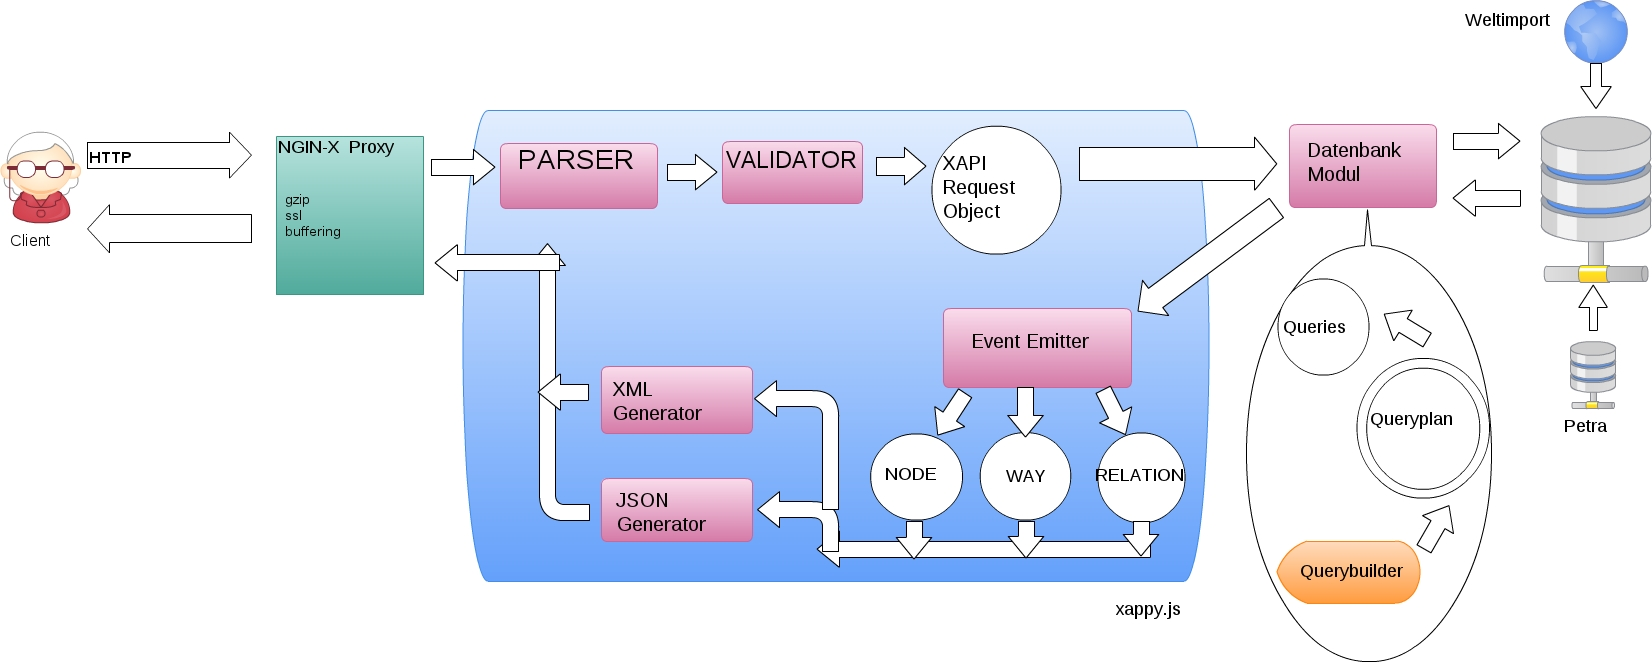
\includegraphics[width=1\textwidth]{../images/xapi.jpg} 
		\caption{Architecture}
		\label{architecture}
	\end{figure}
\end{frame}

\begin{frame}{The Architecture (2)}
	\begin{block}{Modules}
		\begin{itemize}
			\item parser
			\item data base module
			\item XML generator \& JSON generator
			\item event emitter
		\end{itemize}
	\end{block}
\end{frame}

\begin{frame}{The Architecture (3)}
	\begin{block}{Components}
		\begin{itemize}
			\item request structure
			\item internal object
			\item queries
			\item events
			\item output
			\item import
			\item data base scheme
		\end{itemize}
	\end{block}
\end{frame}

%%%%%%%%%%%%%%%%%%%%%%

\section{Work Process}
\begin{frame}{Work Process}
	\begin{itemize}
		\item test driven development
		\item stand up meetings
		\item agile development
		\item collective codebase
		\item CI-system
	\end{itemize}
\end{frame}
\end{document}
